\newpage
\subsection{Ejercicio 3.3: Contrastando con la realidad}

En este punto queremos estimar mediante sucesivos pings el RTT existente entre el host origen \textit{(host desde el cual se realiza el ping)} y cada una de las cuatro universidades elegidas para este trabajo.
En cada ping enviamos un paquete ICMP Echo request y esperamos que el host destino nos responda con el correspondiente paquete ICMP Echo reply. Midiendo el tiempo transcurrido desde que enviamos el echo request hasta que recibimos el echo reply obtenemos una muestra $s_i$ del RTT entre los dos host. Luego, con dicha muestra aplicamos la siguiente fórmula para estimar con mayor fidelidad el RTT de la conexión:
\begin{center}
  $SRTT_{i+1}$ = ($\alpha$ * $SRTT_i$) + (1 - $\alpha$) * $s_i$
\end{center}

Tanto el valor de $\alpha$ como la cantidad de muestras $s_i$ obtenidas son valores que variamos.


Se puede ver que el valor de $\alpha$ controla cuán rápidamente el SRTT se adapta a cambios en la muestra de RTTs. Dado que siempre es posible que una respuesta en particular tarde mucho en llegar \textit{(ya sea por que tomo una ruta más larga que el resto de los paquetes, por un aumento momentáneo de la congestión en la red o por que el host destino retraso el envío de la respuesta)}, consideramos que valores de $\alpha$ por encima de $0.50$ implicarían, prácticamente, ignorar todos los valores muestreados anteriormente. Por este motivo, los valores elegidos para $\alpha$ fueron: $0.15$, $0.30$ y $0.50$.


Por otra parte, elegimos tres tamaños de muestra diferentes: $10$, $70$ y $150$.
Para cada una de las nueves combinaciones posibles entre tamaño de muestra y $\alpha$ estimamos la probabilidad de perdida de paquete como:
\begin{center}
	Probabilidad de perdida de paquetes estimada $=$ $1$ - $\frac{\#Echo\ reply}{\#Echo\ request}$
\end{center}

También calculamos el throughput de la conexión utilizando la fórmula para enlaces ideales, en los casos en que no hubo pérdida de paquetes:
\begin{displaymath}
  throughput = \frac{|Ventana|}{RTT}
\end{displaymath}

En esta fórmula fijamos el valor de $|Ventana|$ en 64 Kbytes.
En los casos en que sí hubo pérdida de paquetes, utilizamos la fórmula de Mathis:
\begin{center}
	throughput < $\frac{MSS}{RTT * \sqrt{p}}$
\end{center}

En dicha fórmula fijamos el valor de MSS \textit{Maximum Segment Size} en 1460 bytes.


A continuación mostraremos, para cada una de las cuatro universidades elegidas, los resultados de la experimentación realizada.

\subsubsection{Universidad Católica de Australia (ACU)}

\begin{figure}[H]
\begin{changemargin}{-5cm}{-5cm}
    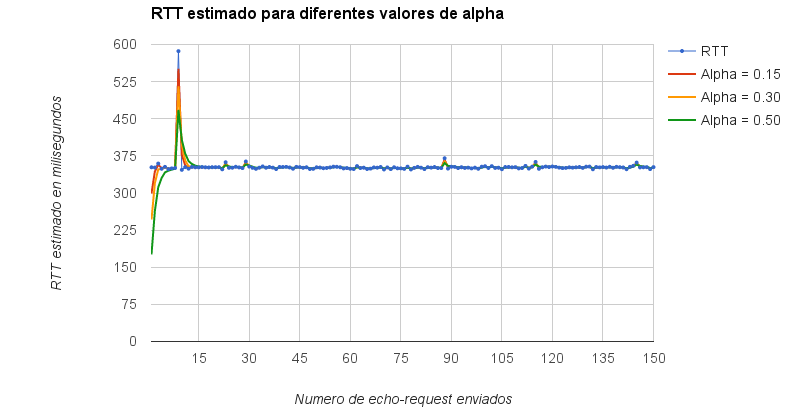
\includegraphics[width=1.5\textwidth]{../Experimentacion/Australia/ertt.png}
    \caption{RTT estimado por cada muestra de RTT para los diferentes valores de $\alpha$}
  \label{ertt-aus}
  \end{changemargin}
\end{figure}


\begin{table}[H]
	\centering
    \begin{tabular}{lllll}
    \hline
    \#Muestras & $\alpha$ & RTT estimado &Prob. estimada perdida paquete & Throughput \\	\hline
    10   &  0.15  &  351.79 ms  &  0.0\%  &  181.9 Kbyte/s  \\
    10   &  0.30  &  351.53 ms  &  0.0\%  &  182.0 Kbyte/s  \\
    10   &  0.50  &  350.73 ms  &  0.0\%  &  182.4 Kbyte/s  \\
    70   &  0.15  &  356.06 ms  &  0.0\%  &  179.7 Kbyte/s  \\
    70   &  0.30  &  354.87 ms  &  0.0\%  &  180.3 Kbyte/s  \\
    70   &  0.50  &  353.43 ms  &  0.0\%  &  181.0 Kbyte/s  \\
    150  &  0.15  &  351.75 ms  &  0.0\%  &  181.9 Kbyte/s  \\
    150  &  0.30  &  351.42 ms  &  0.0\%  &  182.1 Kbyte/s  \\
    150  &  0.50  &  351.38 ms  &  0.0\%  &  182.1 Kbyte/s  \\ \hline
    \end{tabular}
    \caption{Resultado del análisis de las muestras de RTTs para Australia}
  \label{fig:tabla-ertt-aus}
\end{table}


\subsubsection{Universidad de Bergen (UIB) - Noruega}

\begin{figure}[H]
\begin{changemargin}{-5cm}{-5cm}
    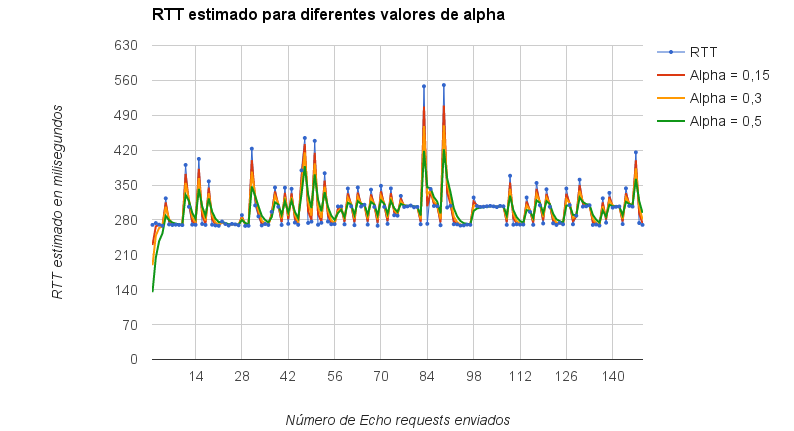
\includegraphics[width=1.5\textwidth]{../Experimentacion/Noruega/ertt.png}
    \caption{RTT estimado por cada muestra de RTT para los diferentes valores de $\alpha$}
  \label{ertt-nor}
\end{changemargin}
\end{figure}

\begin{table}[H]
	\centering
    \begin{tabular}{lllll}
    \hline
    \#Muestras & $\alpha$ & RTT estimado &Prob. estimada perdida paquete & Throughput \\	\hline
    10   &  0.15  &  328.42 ms  &  0.0\%  &  194.8 Kbyte/s  \\
    10   &  0.30  &  335.21 ms  &  0.0\%  &  190.9 Kbyte/s  \\
    10   &  0.50  &  335.69 ms  &  0.0\%  &  190.6 Kbyte/s  \\
    70   &  0.15  &  270.23 ms  &  0.0\%  &  236.8 Kbyte/s  \\
    70   &  0.30  &  272.85 ms  &  0.0\%  &  234.5 Kbyte/s  \\
    70   &  0.50  &  275.58 ms  &  0.0\%  &  229.7 Kbyte/s  \\
    150  &  0.15  &  273.45 ms  &  0.666666666667\%  &  65.4 Kbyte/s  \\
    150  &  0.30  &  281.07 ms  &  0.666666666667\%  &  63.6 Kbyte/s  \\
    150  &  0.50  &  294.13 ms  &  0.666666666667\%  &  60.8 Kbyte/s  \\ \hline
    \end{tabular}
    \caption{Resultado del análisis de las muestras de RTTs para Noruega}
  \label{fig:tabla-ertt-nor}
\end{table}

\subsubsection{Universidad de Tokyo - Japón}

\begin{figure}[H]
\begin{changemargin}{-5cm}{-5cm}
    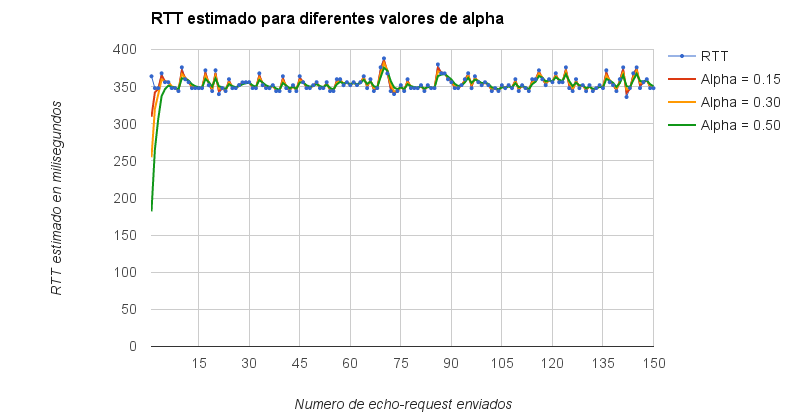
\includegraphics[width=1.5\textwidth]{../Experimentacion/Tokyo/ertt.png}
    \caption{RTT estimado por cada muestra de RTT para los diferentes valores de $\alpha$}
  \label{ertt-tok}
\end{changemargin}
\end{figure}

\begin{table}[H]
	\centering
    \begin{tabular}{lllll}
    \hline
    \#Muestras & $\alpha$ & RTT estimado &Prob. estimada perdida paquete & Throughput \\	\hline
    10   &  0.15  &  307.94 ms  &  0.0\%  &  207.8 Kbyte/s  \\
    10   &  0.30  &  310.33 ms  &  0.0\%  &  206.2 Kbyte/s  \\
    10   &  0.50  &  315.45 ms  &  0.0\%  &  202.8 Kbyte/s  \\
    70   &  0.15  &  295.47 ms  &  5.71428571429\%  &  20.4 Kbyte/s  \\
    70   &  0.30  &  298.96 ms  &  5.71428571429\%  &  20.4 Kbyte/s  \\
    70   &  0.50  &  300.36 ms  &  5.71428571429\%  &  20.3 Kbyte/s  \\
    150  &  0.15  &  299.94 ms  &  4.66666666667\%  &  22.5 Kbyte/s  \\
    150  &  0.30  &  301.54 ms  &  4.66666666667\%  &  22.4 Kbyte/s  \\
    150  &  0.50  &  304.26 ms  &  4.66666666667\%  &  22.2 Kbyte/s  \\ \hline
    \end{tabular}
    \caption{Resultado del análisis de las muestras de RTTs para Rusia}
  \label{fig:tabla-ertt-rus}
\end{table}

\subsubsection{Lomonosov Universidad del estado de Moscú - Rusia}

\begin{figure}[H]
\begin{changemargin}{-5cm}{-5cm}
    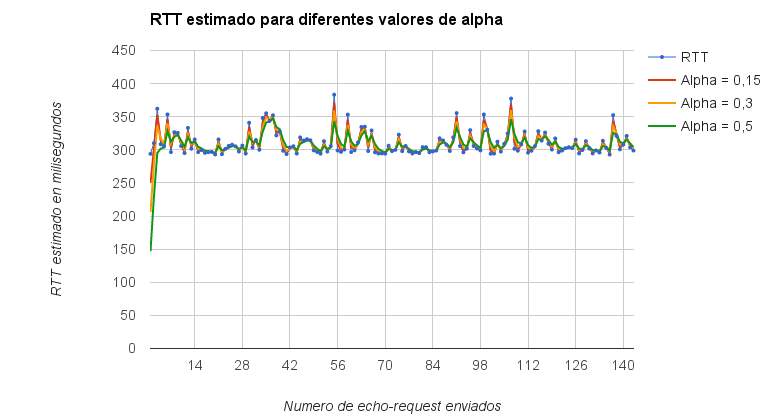
\includegraphics[width=1.5\textwidth]{../Experimentacion/Rusia/ertt.png}
    \caption{RTT estimado por cada muestra de RTT para los diferentes valores de $\alpha$}
  \label{ertt-rus}
\end{changemargin}
\end{figure}

\begin{table}[H]
	\centering
    \begin{tabular}{lllll}
    \hline
    \#Muestras & $\alpha$ & RTT estimado &Prob. estimada perdida paquete & Throughput \\	\hline
    10   &  0.15  &  355.24 ms  &  0.0\%  &  180.1 Kbyte/s  \\
    10   &  0.30  &  355.13 ms  &  0.0\%  &  180.2 Kbyte/s  \\
    10   &  0.50  &  355.14 ms  &  0.0\%  &  180.2 Kbyte/s  \\
    70   &  0.15  &  347.46 ms  &  0.0\%  &  184.1 Kbyte/s  \\
    70   &  0.30  &  347.15 ms  &  0.0\%  &  184.3 Kbyte/s  \\
    70   &  0.50  &  347.15 ms  &  0.0\%  &  184.4 Kbyte/s  \\
    150  &  0.15  &  348.18 ms  &  0.0\%  &  183.8 Kbyte/s  \\
    150  &  0.30  &  348.90 ms  &  0.0\%  &  183.4 Kbyte/s  \\
    150  &  0.50  &  350.55 ms  &  0.0\%  &  182.5 Kbyte/s  \\ \hline
    \end{tabular}
    \caption{Resultado del análisis de las muestras de RTTs para Japon}
  \label{fig:tabla-ertt-tokyo}
\end{table}
